\section{Theory}
\todo{Algorithm for Gibbs sampling}

\todo{Algorithm for contrastive divergence}

\todo{Derivation of log likelihood gradient (appendix)}

\begin{figure}
    \begin{center}
        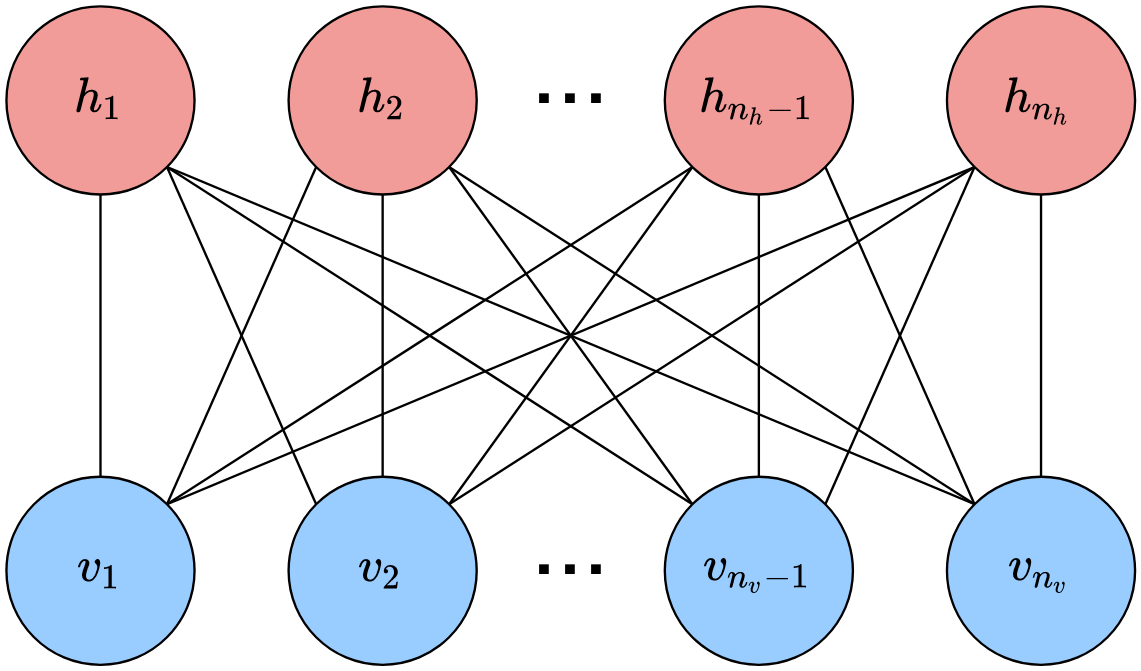
\includegraphics[width=1\linewidth]{rbm_diagram.png}
    \end{center}
    \caption{The structure of a restricted Boltzmann machine with \( n_v \) visible units and \( n_h \) hidden units.}
    \label{fig:rbm_diagram}
\end{figure}

\begin{figure}
    \begin{center}
        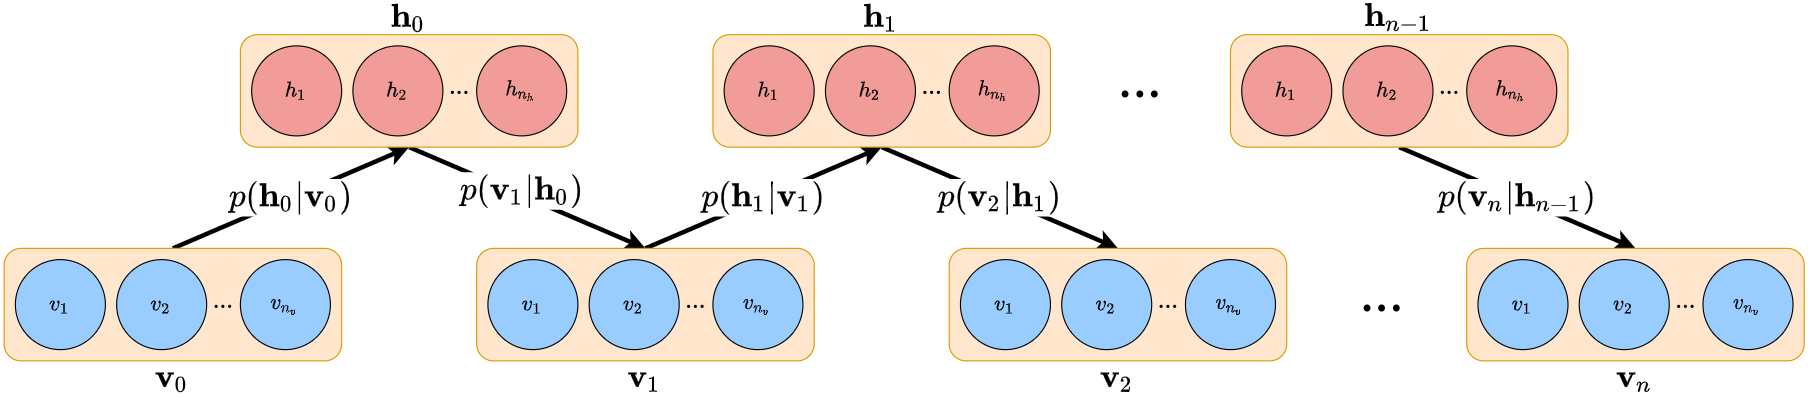
\includegraphics[width=1\linewidth]{gibbs_sampling_diagram.png}
    \end{center}
    \caption{Illustration of the Gibbs sampling procedure.}
    \label{fig:gibbs_sampling_diagram}
\end{figure}

\section{Application}

\section{Results}
In this section we will compare four different RBM models, denoted as:
\begin{itemize}
    \item (B): baseline model.
    \item (V): using volatility indicators.
    \item (X): using a transformed feature space.
    \item (XV): using a transformed feature space and volatility indicators.
\end{itemize}

\begin{table}[ht]
    \centering
    \begin{adjustbox}{max width=\textwidth}
        \input{../tables/rbm/correlation_coefficients.tbl}
    \end{adjustbox}
    \caption{Correlation coefficients of the data vs. samples generated by the RBM models. The RBM numbers are shown in the format average \(\pm\) 1 standard deviation from an ensemble of size 100.}
    \label{tbl:rbm_correlation_coefficients}
\end{table}

\begin{table}[ht]
    \centering
    \begin{adjustbox}{max width=\textwidth}
        \input{../tables/rbm/qq_rmses.tbl}
    \end{adjustbox}
    \caption{QQ root mean squared errors of the RBM models. All numbers are shown in the format average \(\pm\) 1 standard deviation from an ensemble of size 100.}
    \label{tbl:rbm_qq_rmse}
\end{table}

\begin{table}[ht]
    \centering
    \begin{adjustbox}{max width=\textwidth}
        \input{../tables/rbm/volatilities.tbl}
    \end{adjustbox}
    \caption{Historical volatilities of the data vs. samples generated by the RBM models. All numbers are shown in the format average \(\pm\) 1 standard deviation from an ensemble of size 100.}
    \label{tbl:rbm_volatilities}
\end{table}

\begin{table}[ht]
    \centering
    \begin{adjustbox}{max width=\textwidth}
        \input{../tables/rbm/conditional_volatilities.tbl}
    \end{adjustbox}
    \caption{Conditional historical volatilities of the data vs. samples generated by the RBM models. All numbers are shown in the format average \(\pm\) 1 standard deviation from an ensemble of size 100.}
    \label{tbl:rbm_conditional_volatilities}
\end{table}

\begin{table}[ht]
    \centering
    \begin{adjustbox}{max width=\textwidth}
        \input{../tables/rbm/autocorrelation_times.tbl}
    \end{adjustbox}
    \caption{Integrated autocorrelation times of the RBM models.}
    \label{tbl:rbm_ac_times}
\end{table}

\begin{table}[ht]
    \centering
    \begin{adjustbox}{max width=\textwidth}
        \input{../tables/rbm/tails.tbl}
    \end{adjustbox}
    \caption{Lower and upper tails, i.e., 1st and 99th percentiles, of the data vs. samples generated by the RBM models. All numbers are shown in the format average \(\pm\) 1 standard deviation from an ensemble of size 100.}
    \label{tbl:rbm_tails}
\end{table}

\begin{figure}[ht]
    \begin{center}
        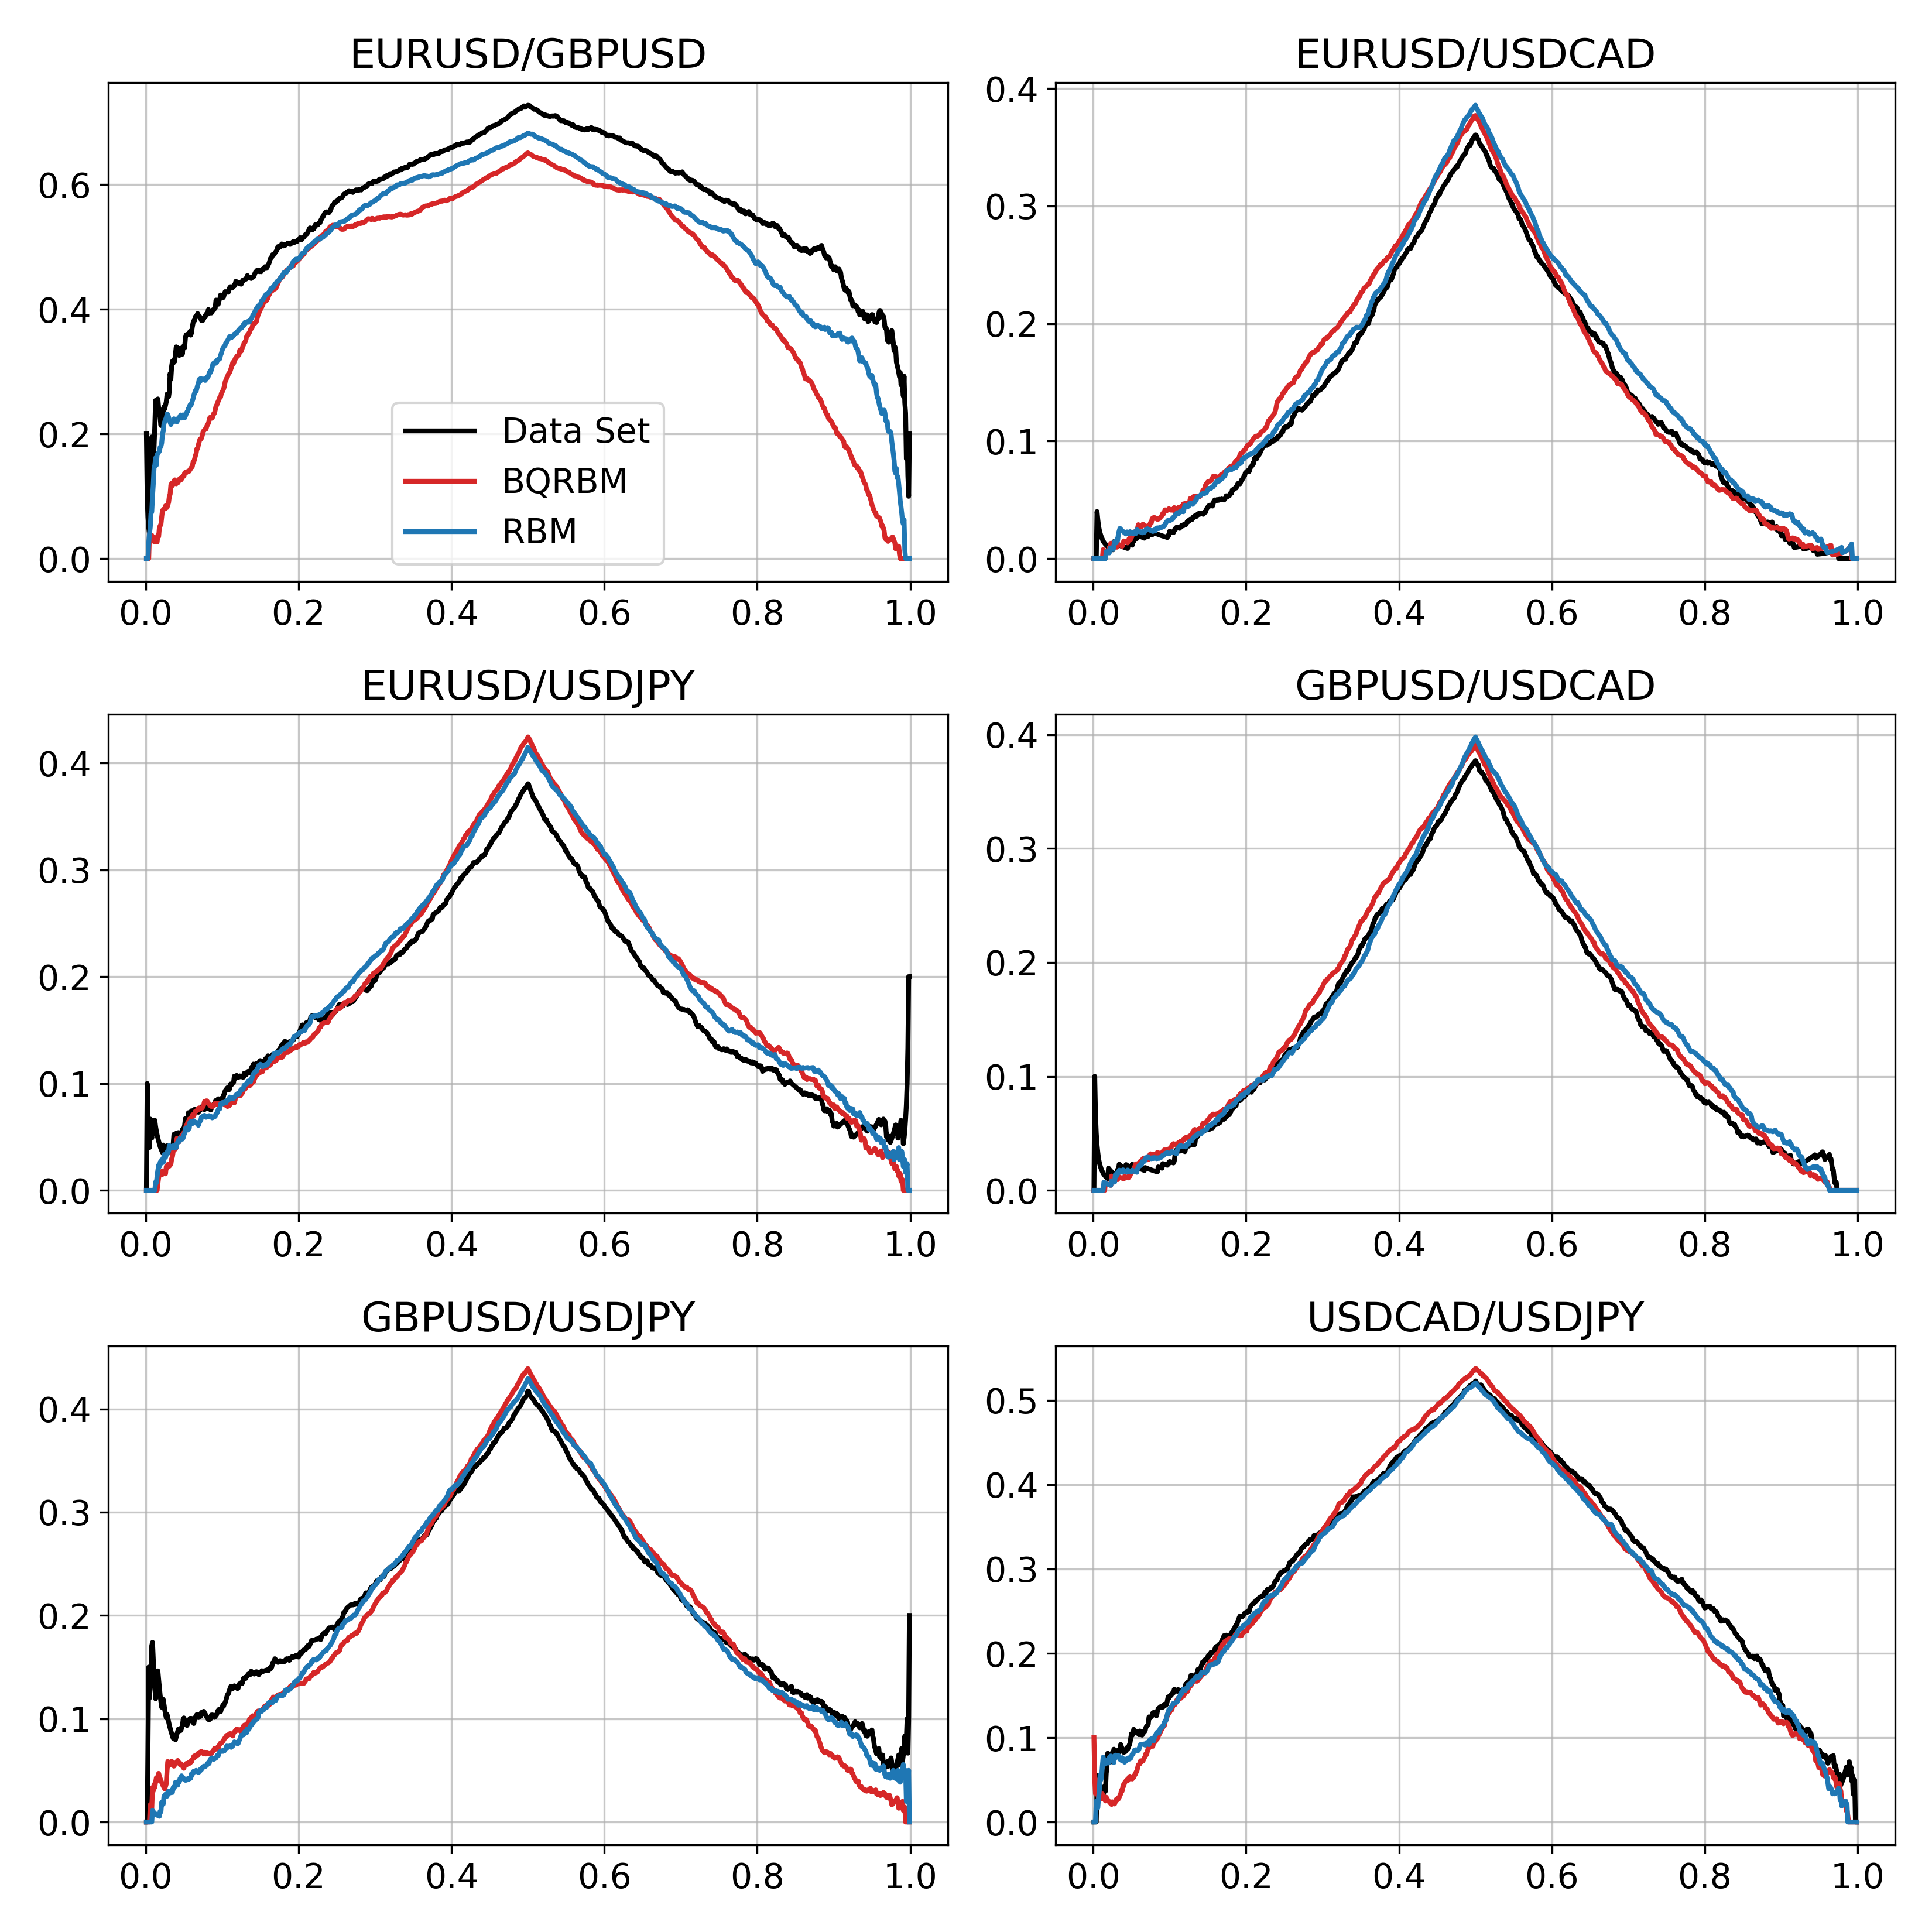
\includegraphics[width=1\linewidth]{rbm/tail_concentrations.png}
    \end{center}
    \caption{Tail concentration functions of the data vs. samples generated by the RBM models.}
    \label{fig:rbm_tail_concentrations}
\end{figure}

\begin{figure}[ht]
    \begin{center}
        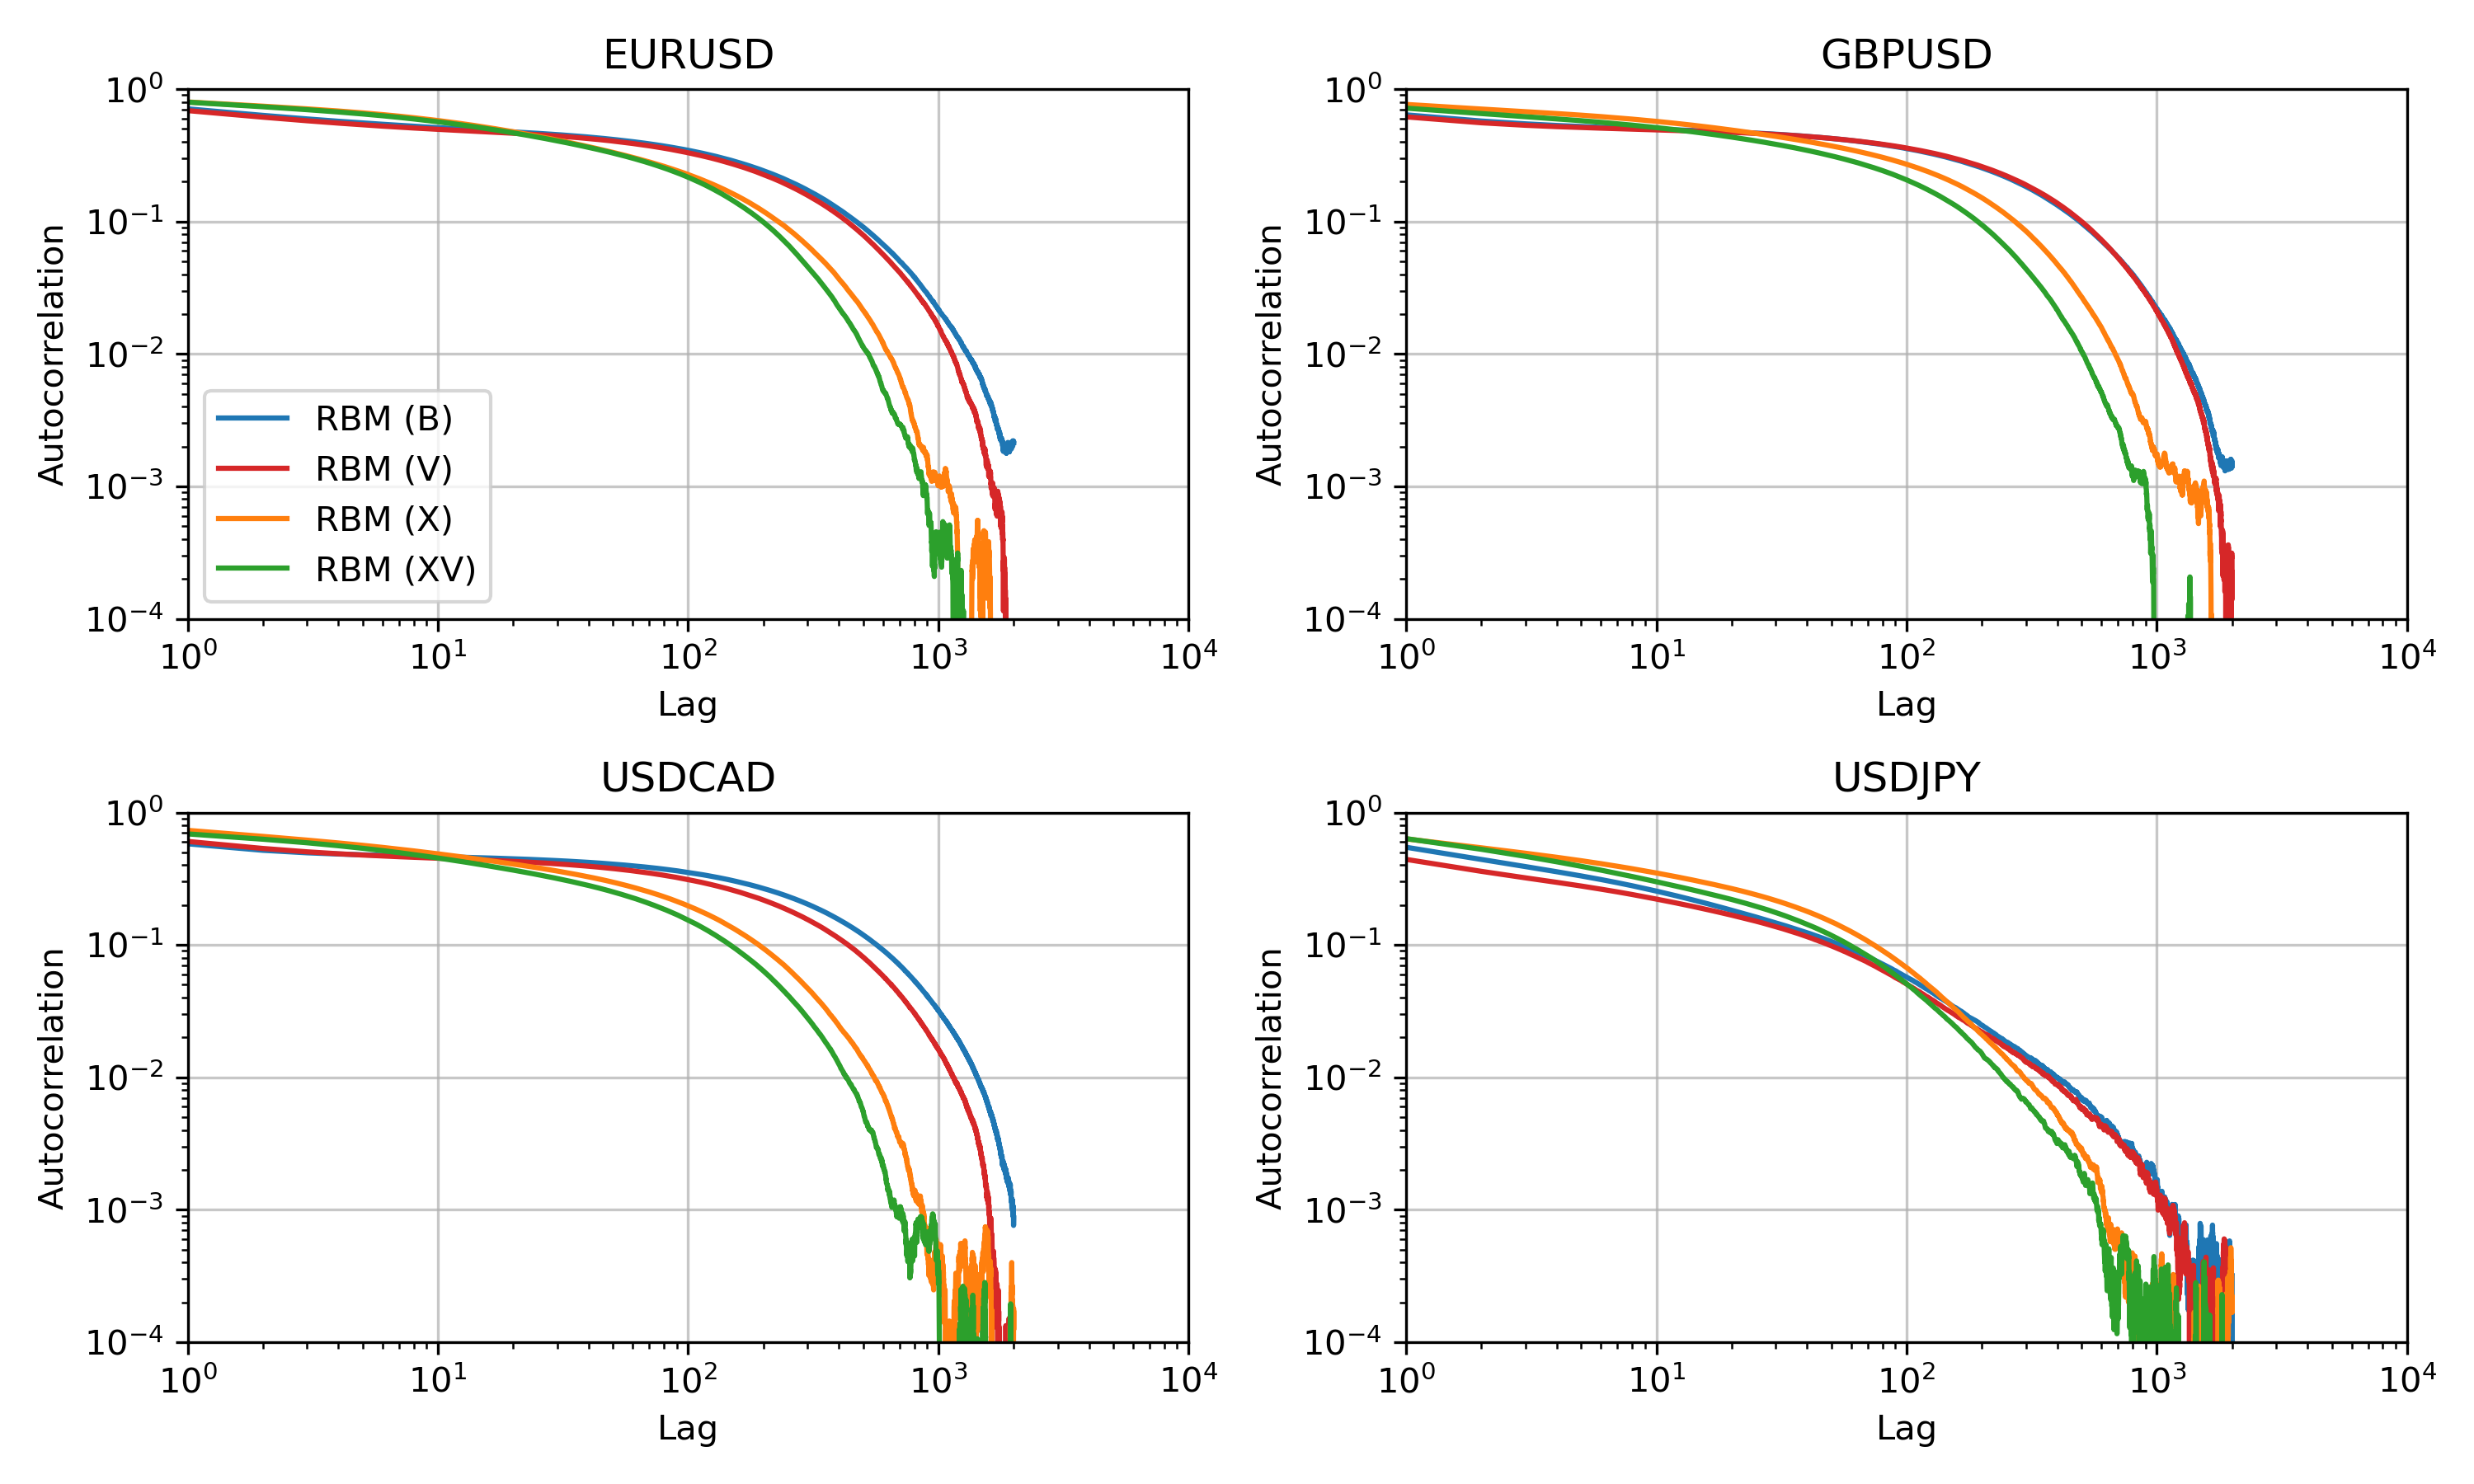
\includegraphics[width=1\linewidth]{rbm/autocorrelation_functions.png}
    \end{center}
    \caption{Autocorrelation functions of the RBM models. Function values are computed from Gibbs sample chains of length \( 10^8 \).}
    \label{fig:rbm_autocorrelation_functions}
\end{figure}

\begin{figure}[ht]
    \begin{center}
        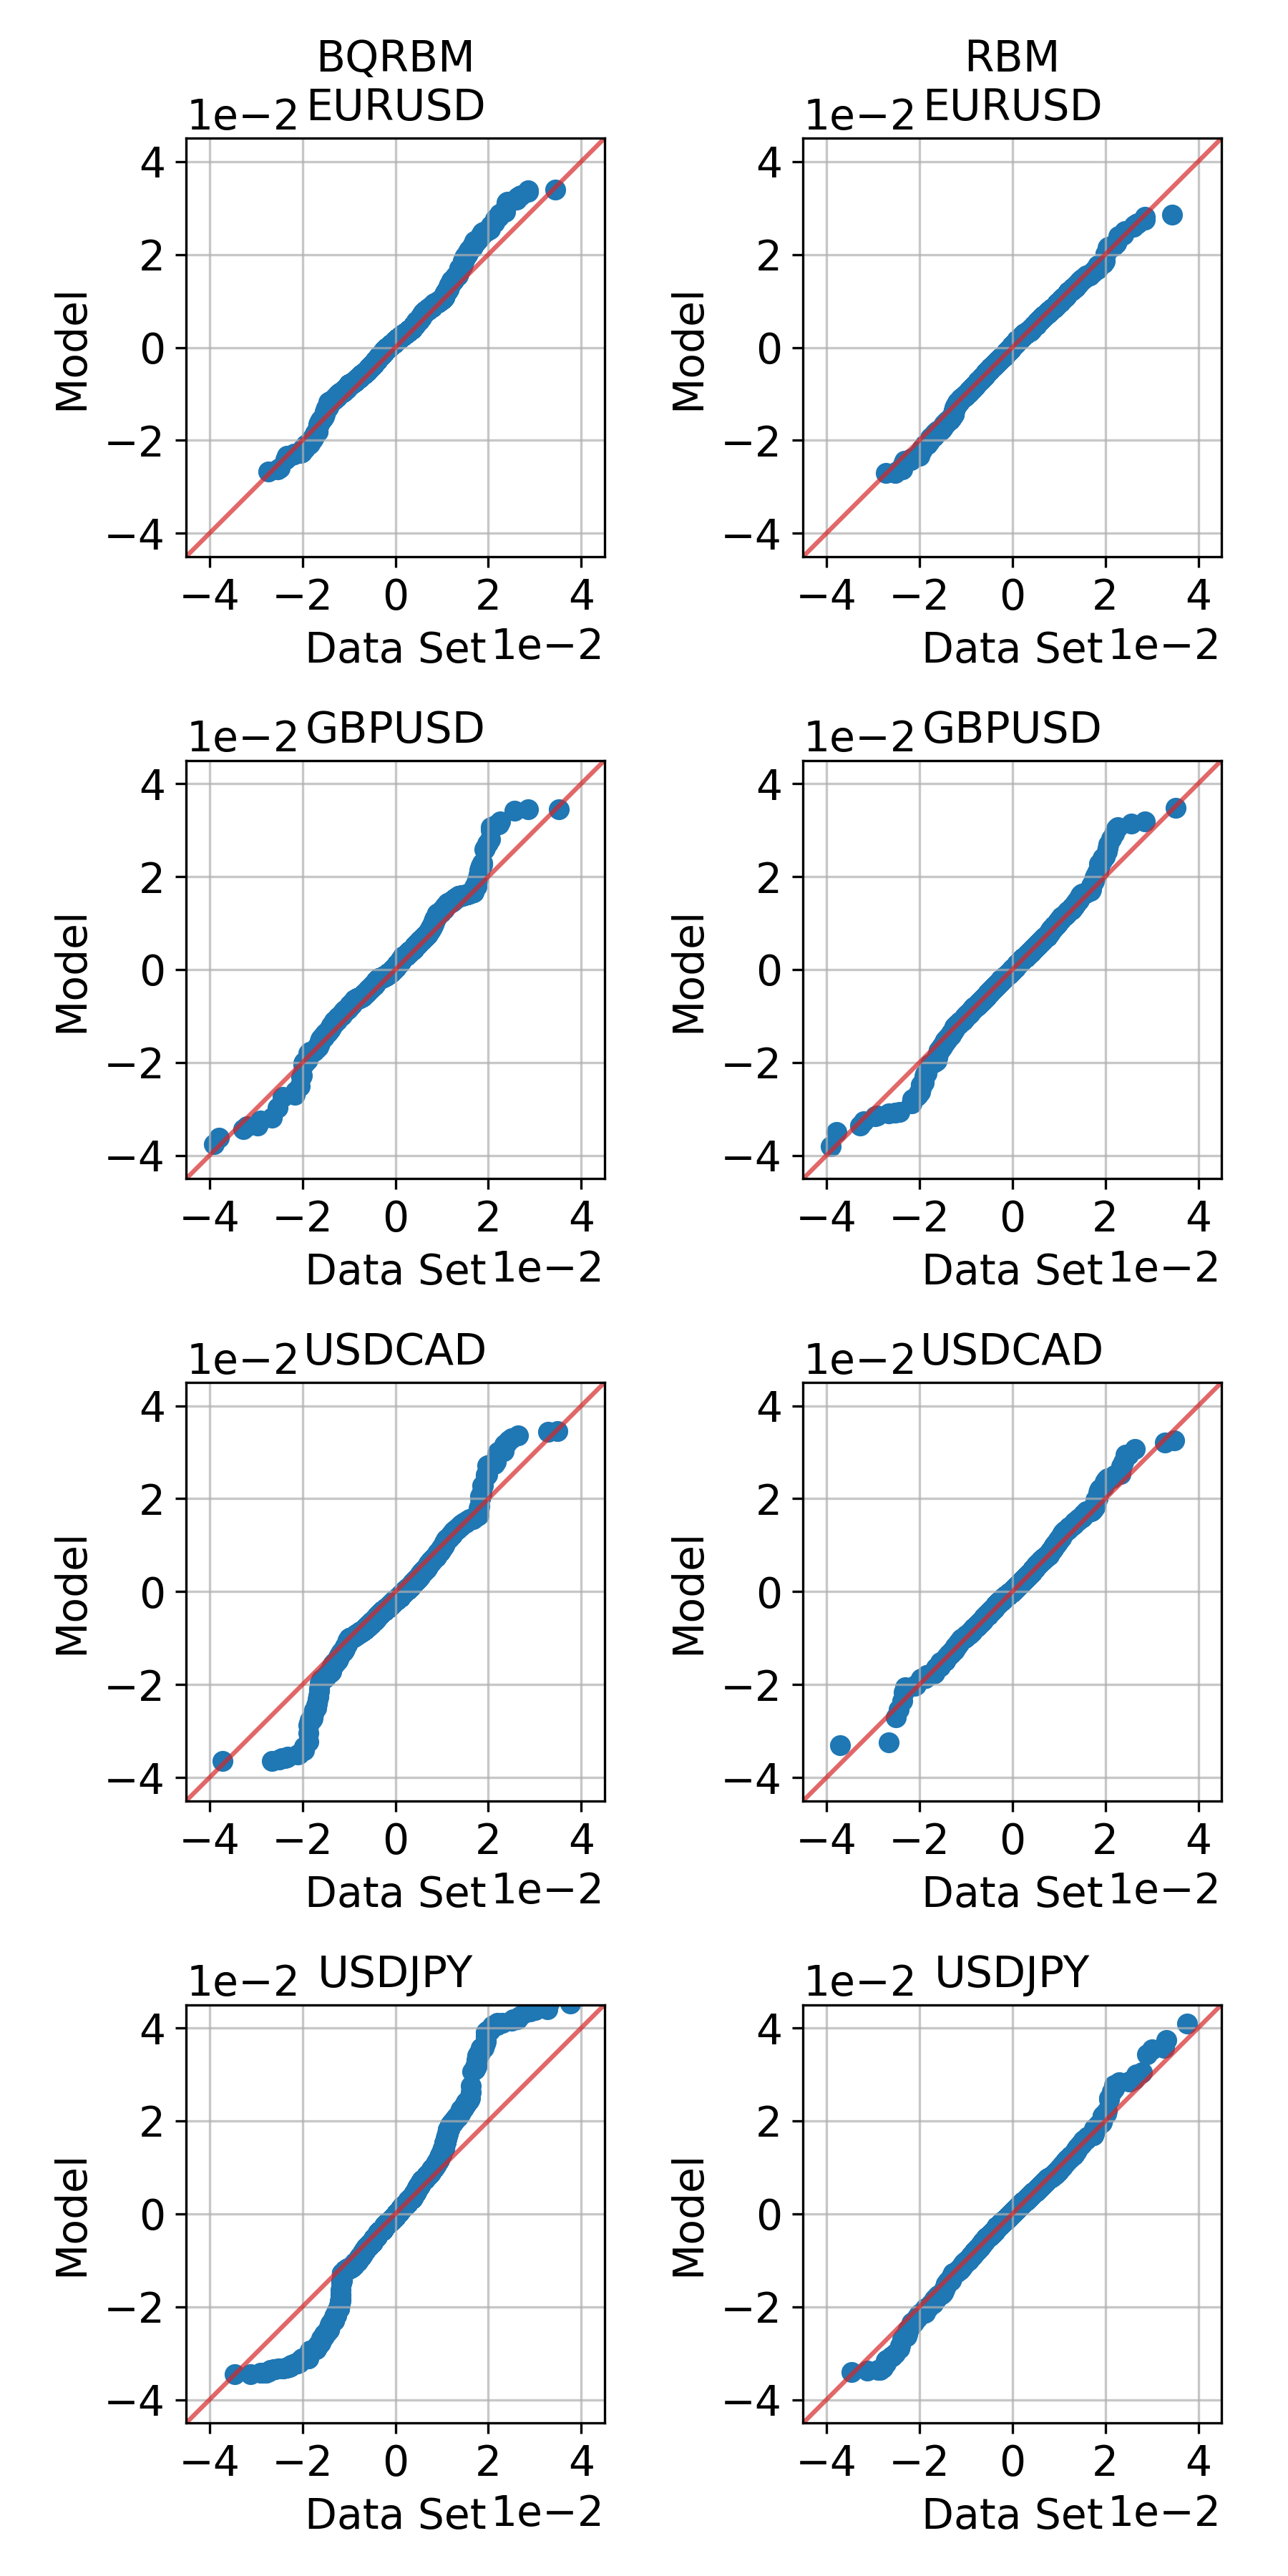
\includegraphics[width=1\linewidth]{rbm/qq.png}
    \end{center}
    \caption{QQ plots of the RBM models.}
    \label{fig:rbm_qq_plots}
\end{figure}
